\documentclass[twocolumn, 11pt]{article}
\usepackage{amsmath, amssymb, amsthm, bm, moresize}
\usepackage{euler}

\usepackage{graphicx, epsdice, xcolor, listings, float, wrapfig, caption}
\usepackage[top=1.2in, bottom=1.2in, left=0.6in, right=0.6in]{geometry}

\usepackage{etoolbox}
\patchcmd{\thebibliography}{\section*{\refname}}{}{}{}

\newcommand{\EE}{\mathbb{E}}
\newcommand{\PP}{\mathbb{P}}
\newcommand{\RR}{\mathbb{R}}
%
\newcommand{\Dd}{\mathcal{D}}
\newcommand{\Ee}{\mathcal{E}}
\newcommand{\Gg}{\mathcal{G}}
\newcommand{\Hh}{\mathcal{H}}
\newcommand{\Ii}{\mathcal{I}}
\newcommand{\Kk}{\mathcal{K}}
\newcommand{\Ll}{\mathcal{L}}
\newcommand{\Ss}{\mathcal{S}}
\newcommand{\Tt}{\mathcal{T}}
\newcommand{\Uu}{\mathcal{U}}
\newcommand{\Vv}{\mathcal{V}}
\newcommand{\Xx}{\mathcal{X}}
\newcommand{\Yy}{\mathcal{Y}}
%
\newcommand{\gG}{\frak{g}}
\newcommand{\oO}{\frak{o}}
\newcommand{\sS}{\frak{s}}


\newcommand{\Ein} {\text{trn}_{\Ss}} %{\Ee_{\text{in},\Uu}}
\newcommand{\Einb} {\text{trn}_{\check\Ss}} %{\Ee_{\text{in},\Uu}}
\newcommand{\Einc} {\text{trn}_{\Ss\sqcup \check\Ss}} %{\Ee_{\text{in},\Uu}}
\newcommand{\Egap}{\text{gap}_{\Ss}}
\newcommand{\Eout}{\text{tst}} %{\Ee_{\text{out}}}

\newtheorem*{qst}{Question}
\newtheorem*{thm}{Theorem}
\newtheorem*{lem}{Lemma}
\newtheorem*{clm}{Claim}
\theoremstyle{definition}
\newtheorem*{dfn}{Definition}

\definecolor{mblu}{rgb}{0.05, 0.40, 0.70}
\newcommand{\msec}[1]{\subsection*{\color{mblu}\textsf{#1}}}

\begin{document}

    \twocolumn[
        \begin{@twocolumnfalse}
            \begin{tabular}{p{0.06\linewidth}p{0.9\linewidth}}
                &
                \begin{flushleft}  \Huge \color{mblu} \bf\textsf{WHAT IS...}    \vspace{0.1cm}\\\hrule  \end{flushleft} \vspace{-1.0\baselineskip}
                \begin{flushright} \HUGE \color{mblu} \bf the Curvature Form?   \end{flushright} \vspace{-1.0\baselineskip}
                \begin{flushright} \Large             \it Samuel C.\ Tenka      \end{flushright}
            \end{tabular}
        \end{@twocolumnfalse}
    ]

    \msec{Connections as Forms}
        If insanity means redoing actions while expecting new results, then
        curvature is a local measure of insanity.

        Let us explain this in the differential geometer's ink-saving world
        where all that can be smooth is smooth and all that can be linear is
        linear.
        %
        A \textbf{connection} on a bundle $\pi:E\to B$ is a
        prescription for how to lift infinitesimal paths through $\pi$.  We may
        lift finite paths by integrating --- this is
        \textbf{transport}.  A connection's \textbf{curvature} measures the
        failure of infinitesimal loops to lift to loops.  Thus, in the presence
        of curvature, the result of traversing a loop $n$ times depends on $n$;
        more generally, transport's destination is path-dependent.

        A connection is a $\tilde\omega: TB \to E \to TE$ where we restrict to
        inputs whose basepoints match and we insist that the output vector
        projects to the input vector.
        %
        Thus, any two connections differ at $v \in T_p B$ by a vector field  
        on $p$'s fiber.
        We may locally choose a flat connection $\tilde\omega_0$ by choosing a
        trivialization of the bundle; relative to $\tilde\omega_0$,
        $\tilde\omega$ has the data of a bunch of vector fields on fibers, 
        comparable between different fibers by means of $\tilde\omega_0$.
        Viewing all those vector fields as living in a Lie algebra $\gG$,
        we may package the data of $\tilde\omega$ as $\omega:TB \to \gG$.
        Note that $\omega$ is only defined locally and depends on a local
        trivialization.



\newpage
    \msec{Curvature as a Form}
        Just as we measure infinitesimal location-dependence using one-forms,
        we measure infinitesimal path-dependence using two-forms.  We therefore
        expect the curvature $\Omega : \Lambda^2 TB \to \gG$ to be a two-form 
        valued in $\gG$.

        Intuitively, there are two obstructions to path-independence:
        (\textbf{horizontal}) the connection might vary with $p$ and  
        (\textbf{vertical}) the vector fields $\omega(\cdot)$ might not
        commute.
        %
        To isolate the horizontal phenomenon, suppose $\gG$ is
        abelian so that transport is just addition in $\gG$.  We then
        want for any disk $h: D^2 \to B$ that
        $$
            \int_{\partial h} \omega = \int_h \Omega
        $$
        In this case, we must take $\Omega = d\omega$.
        %
        To isolate the vertical phenomenon, suppose $\omega$ is closed, i.e.\
        in local coordinates constant.  Then for an
        infinitesimal rectangle in these coordinates with sides $u, v$, we
        want:
        $$
            e^{\omega(-u)}e^{\omega(-v)}e^{\omega(v)}e^{\omega(u)}
            =
            e^{\Omega(u,v)}
        $$
        In this case, we must take $\Omega(u,v) = [\omega(u), \omega(v)]$.
        %
        The general expression for \textbf{curvature} is a sum:
        $$
            \Omega(u,v) = d\omega(u,v) + [\omega(u), \omega(v)]
        $$

        For example, a Riemannian manifold $B$ of dimension $d$ has a bundle of
        orthonormal bases; the relevant algebra is $\oO(d)$.  Then
        $\Omega:\Lambda^2 TB \to \oO(d)$ has the same data as the Riemann
        tensor, and it emphasizes the variance and antisymmetry of the indices. 

    \newpage
    \msec{Chern's Gauss-Bonnet}
        Chern proved the Gauss-Bonnet Theorem using the curvature form for the
        bundle $UB$ of unit vectors on a (compact oriented) surface $B$. 

        The key insight is to lift this form by   

        Fix a vector field on $B$ with one non-degenerate zero at $p$.
        By Poincar\'e-Hopf, the zero has degree $\chi(B)$. 
        Regard the graph of the normalized vector field as a smooth
        submanifold $M$ of $U(B - \{p\})$; the boundary of $M$ winds around
        the $S^1$-shaped fiber $\chi(B)$ times.

        Then
        $$
            \int_B \Omega = \int_M \Omega
                          = \int_{\partial M} \omega
                          = \chi(B) \cdot \int_{S^1} \omega
        $$
        We finish by observing that $\int_{S^1} \omega = 2\pi$.

        Using double covers, we deduce that G-B also applies to non-orientable
        manifolds.

        \newpage
    \msec{A Useful Holonomy}
        It is observed with awe that certain pets, upon falling, land always on
        their feet.  Due to dander allergies, we will imagine a falling cow.

    \msec{Forms are Fun}
        There is much beyond this tiny tour.  We will not mention, for
        instance, how a connection on a circle bundle elegantly describes
        light, its curvature form containing as components both the electric
        and magnetic fields.  Nor will we remark that Chern's proof immediately
        generalizes beyond surfaces, thus relating geometry and topology in all
        even dimensions. 

    \msec{References}
        We thank \textsc{Professor Ralf Spatzier} for teaching us to love
        pictures.

        \hrulefill
        \vspace{0.4cm}
            \begin{wrapfigure}{r}{3.3cm}
                \vspace{-0.4cm}
                    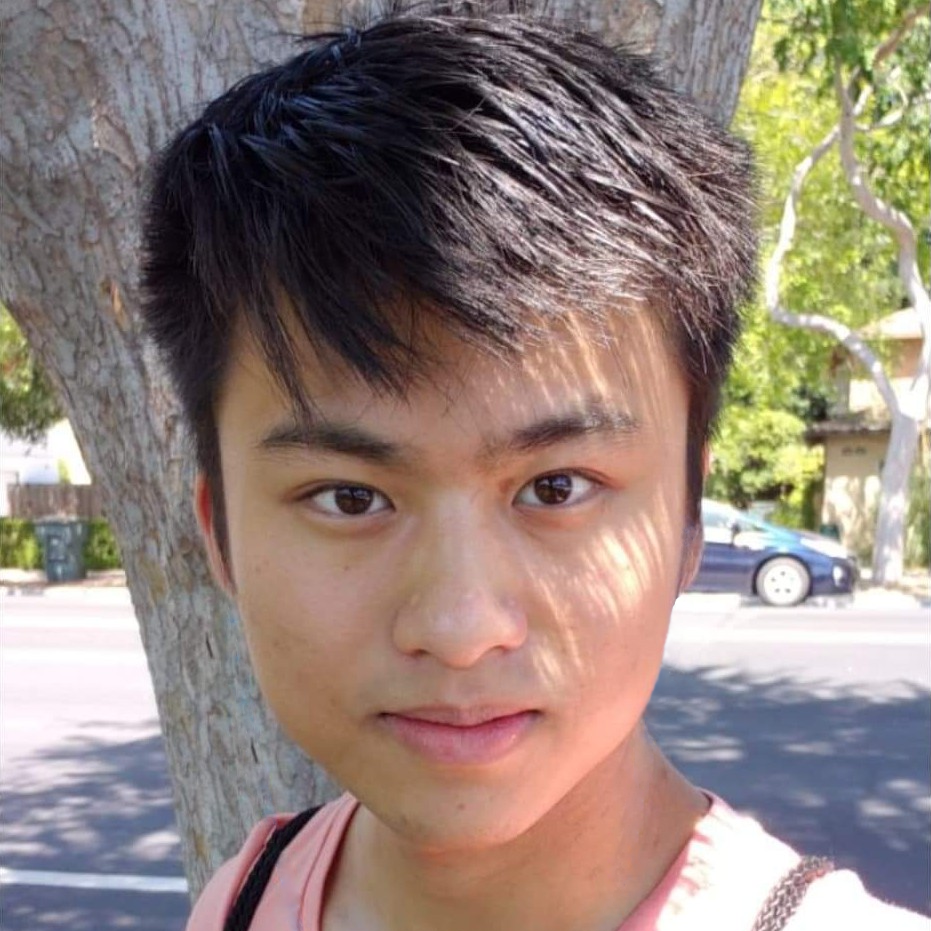
\includegraphics[height=3.3cm]{sam}
                \caption*{The author, courtesy of Karl Winsor}
            \end{wrapfigure}
            When not thinking about machines that learn, Sam can often be found
            pretending to be a cow.  Sam enjoys memory over experience, pet
            snails over pet spinach, left adjoints over right adjoints, and
            analogies over lists.


\end{document}


